\documentclass[12pt,english,brazil,a4paper,utf8,oneside]{utfpr-tcc}

% carrega o arquivo configuracoes.tex que contém os pacotes e comandos Latex.
%
% Esse arquivo conterá pacotes e comandos utilizados na monografia
%
% Observação - devido a um erro do sharelatex foi necessário colocar na raiz do projeto os seguintes arquivos:
% gcnumparser.sty, fcprefix.sty, fmtcount.sty, fc-poruges.def, fcportuguese.def.
% Tal problema foi relatado em: https://github.com/nlct/fmtcount/issues/26
% Quando o sharelatex corrigir o problema acredito que podemos remover esses arquivos do projeto. At. Luiz Arthur.
%

% Este comando não é necessário: utilizei apenas para deixar o latex2rtf
% feliz (e descobrir a codificação do texto).
\usepackage[utf8]{inputenc}

% Suporte a figuras e subfiguras
\usepackage{graphics}
\usepackage{subfigure}

% Suporte a tabelas (principalmente do cronograma)
\usepackage{tabularx}
\usepackage{multirow}
\usepackage{array}
\usepackage{tabularx}
\usepackage{colortbl}
\usepackage{hhline}
\usepackage{xcolor}

% Escalar fontes para redimencionar, por exemplo tabelas
\usepackage{scalefnt}

% Algoritmos.
\usepackage{algorithm,algorithmic}

\usepackage[alf]{abntex2cite}

% Elementos geralmente utilizados na tabela do cronograma
\newcommand{\fullcell}{\multicolumn{1}{>{\columncolor[gray]{0.5}}c}{}}
\newcommand{\fullcellline}{\multicolumn{1}{>{\columncolor[gray]{0.5}}c|}{}}
\newcommand{\mc}[3]{\multicolumn{#1}{#2}{#3}}
\newcommand{\y}{\rule{8pt}{4pt}}
\newcommand{\n}{\hspace*{8pt}}


% Define o caminho das figuras
\graphicspath{{images/}}

%% Configuração de glossário
\usepackage[portuguese]{nomencl}
\usepackage[nogroupskip,acronym,nomain,nonumberlist,nopostdot,nohypertypes={acronym}]{glossaries}

\makenoidxglossaries

% para siglas em português
\newcommand{\sigla}[2]
{
 \newglossaryentry{#1}{
  name=#1,
  description={#2},
  first={#2 (#1)},
  long={#2}
 }  
}

% para siglas de língua estrangeira, nessas a descrição longa fica em itálico.
\newcommand{\siglaIt}[2]
{
 \newglossaryentry{#1}{
  name=#1,
  description={\textit{#2}},
  first={\textit{#2} (#1)},
  long={\textit{#2}}
 }  
}

% --- Estilos para apresentação de Código ----- %
\usepackage{listings}
\lstloadaspects{formats}

% Opções de listing usados para o código fonte
% Ref: http://en.wikibooks.org/wiki/LaTeX/Packages/Listings

\lstset{ %
language=Java,                  % choose the language of the code
basicstyle=\footnotesize,       % the size of the fonts that are used for the code
%basicstyle=\ttfamily,
stringstyle=\ttfamily\color[rgb]{0.16,0.16,0.16},
numbers=left,                   % where to put the line-numbers
numberstyle=\footnotesize,      % the size of the fonts that are used for the line-numbers
stepnumber=1,                   % the step between two line-numbers. If it's 1 each line will be numbered
numbersep=4pt,                  % how far the line-numbers are from the code
showspaces=false,               % show spaces adding particular underscores
showstringspaces=false,         % underline spaces within strings
showtabs=false,                 % show tabs within strings adding particular underscores
frame=single,	                % adds a frame around the code
framerule=0.6pt,
tabsize=2,	                % sets default tabsize to 2 spaces
captionpos=b,                   % sets the caption-position to bottom
breaklines=true,                % sets automatic line breaking
breakatwhitespace=false,        % sets if automatic breaks should only happen at whitespace
escapeinside={\%*}{*)},         % if you want to add a comment within your code
backgroundcolor=\color[rgb]{1.0,1.0,1.0}, % choose the background color.
rulecolor=\color[rgb]{0.8,0.8,0.8},
extendedchars=true,
xleftmargin=10pt,
xrightmargin=10pt,
framexleftmargin=10pt,
framexrightmargin=10pt
}

\definecolor{javared}{rgb}{0.6,0,0} % for strings
\definecolor{javagreen}{rgb}{0.25,0.5,0.35} % comments
\definecolor{javapurple}{rgb}{0.5,0,0.35} % keywords
\definecolor{javadocblue}{rgb}{0.25,0.35,0.75} % javadoc

\definecolor{DarkBlue}{rgb}{0,0,0.61}
\definecolor{DarkGreen}{rgb}{0,0.4,0}

% Numeros.
\lstdefinestyle{mynumbers}{
	numbers=left,
	stepnumber=1,
	numbersep=4pt,
	numberstyle=\tiny\color{black}
}
% Text Code.
\lstdefinestyle{mytextcode}{
	basicstyle=\footnotesize,
	tabsize=2,
	showspaces=false,
	showstringspaces=false,
	extendedchars=true,
	breaklines=true
}
% Frame.
\lstdefinestyle{myframe}{
	backgroundcolor=\color{white},
	frame=trbl
}
% C++ Style.
\lstdefinestyle{C++}{
	language=C++,
	style=mynumbers,
	style=mytextcode,
	style=myframe,
  keywordstyle=\color{black}\bfseries,
  stringstyle=\color{gray},
  commentstyle=\color[rgb]{0.08,0.08,0.08},
  morecomment=[s][\color{lightgray}]{/*}{*/},
  otherkeywords={\#include, \#define, \#pragma, \#typedef, dim3},
  emph={ __device__, __global__, __shared__, __host__, __constant__},
  emphstyle=\color{DarkBlue}\bfseries,
  emph={[2] printf, scanf},
  emphstyle=[2]\color{DarkGreen},
}
% C Style.
\lstdefinestyle{C}{
	language=C,
	style=mynumbers,
	style=mytextcode,
	style=myframe,
	keywordstyle=\color{black}\bfseries,
  	stringstyle=\color{gray},
  	commentstyle=\color[rgb]{0.08,0.08,0.08},
  	morecomment=[s][\color{lightgray}]{/*}{*/},
  	otherkeywords={\#include, \#define, \#pragma, \#typedef, dim3, bool},
  	emph={ __device__, __global__, __shared__, __host__, __constant__},
  	emphstyle=\color{DarkBlue}\bfseries,
  	emph={[2] printf, scanf},
  	emphstyle=[2]\color{DarkGreen},
	backgroundcolor={}
}
% Bash Style.
\lstdefinestyle{bash}{
	language=bash,
	style=mynumbers,
	style=mytextcode,
	style=myframe,
	backgroundcolor={},
	frame=single,
	basicstyle=\scriptsize\ttfamily
}
% Python Style.
\lstdefinestyle{python}{
	language=python,
	style=mynumbers,
	style=mytextcode,
	style=myframe,
	backgroundcolor={}
}
% Java Style.
\lstdefinestyle{java}{
	language=java,
	style=mynumbers,
	style=mytextcode,
	style=myframe,
	backgroundcolor={}
}
% ASM Style.
\lstdefinestyle{asm}{
  %belowcaptionskip=1\baselineskip,
  %xleftmargin=\parindent,
  language=[x86masm]Assembler,
  style=mynumbers,
  style=mytextcode,
  style=myframe,
  backgroundcolor={},
  frame=single,
  basicstyle=\scriptsize\ttfamily,
  commentstyle=\itshape\color{purple!40!black},
}

% Fortran Style.
\lstdefinestyle{fortran}{
  language=[90]Fortran,
  style=mynumbers,
  style=mytextcode,
  style=myframe,
  backgroundcolor={},
  frame=single,
  basicstyle=\footnotesize,
  commentstyle=\itshape\color{purple!40!black},
  morecomment=[l]{!\ }% Comment only with space after !
}



% LLVM Style.
\lstdefinestyle{llvm}{
	language=llvm,
	%inputencoding=utf8,
	style=mynumbers,
	style=mytextcode,
	style=myframe,
	backgroundcolor={},
	frame=single,
	basicstyle=\scriptsize\ttfamily,
  tabsize=4,
  %rulecolor=,
  upquote=true,
% aboveskip={1.5\baselineskip},
  columns=fixed,
  prebreak = \raisebox{0ex}[0ex][0ex]{\ensuremath{\hookleftarrow}},
  showtabs=false,
	%basicstyle=\scriptsize\upshape\ttfamily,
  identifierstyle=\ttfamily,
  keywordstyle=\ttfamily\bfseries\color[rgb]{0,0,0},
  %commentstyle=\ttfamily\color[rgb]{0.133,0.545,0.133},
  commentstyle=\ttfamily\color[rgb]{0.08,0.08,0.08},
  %stringstyle=\ttfamily\color[rgb]{0.627,0.126,0.941}
  stringstyle=\ttfamily\color[rgb]{0.16,0.16,0.16}
}
\newcommand\JSONnumbervaluestyle{\color{blue}}
\newcommand\JSONstringvaluestyle{\color{red}}

% switch used as state variable
\newif\ifcolonfoundonthisline

\makeatletter

\lstdefinestyle{json}
{
  showstringspaces    = false,
  keywords            = {false,true},
  alsoletter          = 0123456789.,
  morestring          = [s]{"}{"},
  stringstyle         = \ifcolonfoundonthisline\JSONstringvaluestyle\fi,
  MoreSelectCharTable =%
    \lst@DefSaveDef{`:}\colon@json{\processColon@json},
  basicstyle          = \ttfamily,
  keywordstyle        = \ttfamily\bfseries,
}

% flip the switch if a colon is found in Pmode
\newcommand\processColon@json{%
  \colon@json%
  \ifnum\lst@mode=\lst@Pmode%
    \global\colonfoundonthislinetrue%
  \fi
}

\lst@AddToHook{Output}{%
  \ifcolonfoundonthisline%
    \ifnum\lst@mode=\lst@Pmode%
      \def\lst@thestyle{\JSONnumbervaluestyle}%
    \fi
  \fi
  %override by keyword style if a keyword is detected!
  \lsthk@DetectKeywords% 
}

% reset the switch at the end of line
\lst@AddToHook{EOL}%
  {\global\colonfoundonthislinefalse}

\makeatother



\lstdefineformat{C}{%
	\{=\newline\string\newline\indent,%
	\}=[;]\newline\noindent\string\newline,%
	\};=\newline\noindent\string\newline,%
	;=[\ ]\string\space}

% --- Fim da Definição de Estilos para apresentação de Código ----- %
% carrega o arquivo constantes.tex que contém dados do curso/monografia que NÃO DEVEM ser alterados. 
% Dados do curso que não precisam de alteração
\university{Universidade Tecnológica Federal do Paraná}
\universityen{Federal University of Technology -- Paraná}
\universityunit{Departamento Acadêmico de Computação}
\address{Campo Mourão}
\addressen{Campo Mourão, PR, Brazil}
\documenttype{Monografia}
\documenttypeen{Monograph}
\degreetype{Graduação}
% carrega o arquivo variaveis.tex que contém dados do acadêmico/monografia que DEVEM ser alterados.
% Dados do curso. Caso seja BCC:
\program{Curso de Bacharelado em Ciência da Computação}
\programen{Undergradute Program in Computer Science}
\degree{Bacharel}
\degreearea{Ciência da Computação}
% Caso seja TSI:
% \program{Curso Superior de Tecnologia em Sistemas para Internet}
% \programen{Undergradute Program in Tecnology for Internet Systems}
% \degree{Tecnólogo}
% \degreearea{Tecnologia em Sistemas para Internet}


% Dados da disciplina. Escolha uma das opções e a descomente:
% TCC1:
\goal{Proposta de Trabalho de Conclusão de Curso de Graduação}
\course{Trabalho de Conclusão de Curso 1}
% TCC2:
% \goal{Trabalho de Conclusão de Curso de graduação}
% \course{Trabalho de Conclusão de Curso 2}


% Dados do TCC (precisa alterar)
\author{Emanuel Felipe Giroldo Mazzer}  % Seu nome
\title{Arquitetura para auxiliar na detecção e visualização de vulnerabilidades em redes de computadores} % Título do trabalho
\titleen{} % Título traduzido para inglês
\advisor{Prof. Dr. Luiz Arthur Feitosa Santos} % Nome do orientador. Lembre-se de prefixar com "Prof. Dr.", "Profª. Drª.", "Prof. Me." ou "Profª. Me."}
% \coadvisor{} % Nome do coorientador, caso exista. Caso não exista, comente a linha.
\depositshortdate{2017} % Ano em que depositou este documento

% Dados da ficha catalografica. Ela é opcional, mas é uma boa ideia inserí-la. Exemplos para geração (http://fichacatalografica.sibi.ufrj.br/)
\fichacatautor{Mazzer, Emanuel F. G}  % Nome conforme citado (ou seja, no formato "Sobrenome, Nome").
\fichacatbib{Biblioteca da UTFPR de Campo Mourão} % Não alterar
\fichacatpum{M488} % Código Cutter-Sanborn. Use a primeira letra do sobrenome seguido do número conforme as primeiras letras do sobrenome e a tabela http://www.amormino.com.br/cutter-sanborn/cutter1.html
\fichacatpalcha{} % Assuntos do trabalho. Cada item deve ser enumerado e separado por ponto: 1. xxx. 2. yyy. 3. zzz.
\fichacatpdois{} % Deixar em branco

% carrega o arquivo listaabreviaturas.tex que está dentro do diretório pretextual, esse arquivo contém as siglas utilizadas na monografia.
% quando a sigla for de língua portuguesa utilize \sigla{SIGLA}{Significado em português}
% quando a sigla for de língua estrangeira utilize \siglaIt{SIGLA}{Significado em Inglês}

\sigla{UTFPR}{Universidade Tecnológica Federal do Paraná}
\siglaIt{pentest}{Penetration testing}
\siglaIt{ACM}{Association for Computing Machinery}
\siglaIt{IP}{Internet Protocol}
\siglaIt{SQL}{Structured Query Language}
\siglaIt{PHP}{Personal Home Page}
\siglaIt{OpenVAS}{Open Vulnerability Assessment System}
\siglaIt{SVM}{Session manegement vulnerabilities}
\siglaIt{URL}{Uniform Resource Locator}
\siglaIt{SID}{Session Identifier}
\siglaIt{CSRF}{Cross-Site Request Forgery}
\siglaIt{GSA}{Greenbone Security Assistant}
\siglaIt{OMP}{OpenVAS Manegement Protocol}
\siglaIt{OTP}{OpenVAS Transfer Protocol}
\siglaIt{NVT}{Network Vulnerability Tests}
\siglaIt{NASL}{Nessus Attack Scripting Language}
\siglaIt{GPL}{General Public Licence}
\siglaIt{HTML}{HyperText Markup Language}
\siglaIt{XML}{eXtensible Markup Language}
\siglaIt{JSON}{JavaScript Object Notation }
\siglaIt{CVSS}{Common Vulnerability Scoring System}
\siglaIt{CVE}{Common Vulnerabilities and Exposures}
\siglaIt{SQLI}{SQL Injection}
\siglaIt{Nmap}{Network mapper}
\siglaIt{MAC}{Media Access Control}
\siglaIt{OS}{Operating System}
\newcommand{\hst}{\textit{host}}
\newcommand{\hsts}{\textit{hosts}}



% No texto quando for utilizar a sigla utilize os seguintes comandos:
%\acrlong{label} - acronimo/sigla longo
%\acrshort{label} - acronimo/sigla curta
%\Gls{TCP} - sigla com o significado primeiro em Maiusculo
%\GLS{TCP} - sigla com o significado tudo em MAIUSCULO
%\gls{TCP} - sigla com o significado tudo em minusculo % usando glossaries

\begin{document}
	
\frontmatter
\maketitle

% carrega o arquivo resumo.tex que está dentro do diretório pretextual, esse arquivo deve conter o resumo da monografia.
\begin{resumo}
%Elemento obrigatório, constituído de uma sequência de frases concisas e objetivas, em forma de texto.  Deve apresentar os objetivos, métodos empregados, resultados e conclusões.  O resumo deve ser redigido em parágrafo único, conter no máximo 500 palavras e ser seguido dos termos representativos do conteúdo do trabalho (palavras-chave).

A Internet vem se tornando cada vez mais popular e indispensável para a maioria da população. Hoje a Internet é uma das maiores fontes de informações, utilizada para a realização de diversas atividades do dia a dia, tais como: transações bancárias, compras \textit{online}, entre outras. Porém  é necessário garantir a segurança dos dados que trafegam tanto na Internet como em quaisquer outras redes de computadores. Para que a segurança dos dados ocorram, vulnerabilidades existentes em dispositivos  conectados à rede devem ser encontradas e corrigidas, mas a detecção de vulnerabilidades nem sempre é uma tarefa simples, pois na maioria das vezes, vulnerabilidades estão contidas em softwares de terceiros, ou até mesmo nas configurações das redes, realizadas pelos próprios administradores e podem acabar passando despercebidas. Entretanto, existem programas que são utilizados para analisar os dispositivos conectados na rede em busca de informações, tais programas são chamados de \textit{scanners}, e podem auxiliar no gerenciamento de redes de computadores. No entanto, quando as redes possuem centenas de dispositivos conectados, os \textit{scanners} tendem a retornar grandes quantidades de informações, demandando um grande tempo para que os administradores analisem as informações, testem as vulnerabilidades encontradas e caso sejam confirmadas, corrijam tais vulnerabilidades.
Dessa maneira, este trabalho propõe uma arquitetura capaz de auxiliar na detecção e visualização de vulnerabilidades em redes de computadores. Sensores serão utilizados com o objetivo de obter a maior quantidade de informações disponíveis a respeito dos dispositivos que serão analisados. Tais informações serão utilizadas para criar perfis para os dispositivos da rede. Estes perfis serão armazenadas, criando uma base de dados contendo todas as informações obtidas. Essas informações serão utilizadas para auxiliar o usuário na administração da rede, as informações podem ser mostrada de maneira gráfica, através de uma interface web, facilitando o entendimento dos resultados obtidos. Além disso, para validar a arquitetura proposta será implementada uma ferramenta, na qual será utilizada dois \textit{scanners} para obter informações a respeito da rede analisadas. As informações obtidas serão utilizadas para auxiliar no gerenciamento e manutenção da rede monitorada. 
É esperado que a arquitetura consiga lidar com grandes quantidades de informações obtidas a partir da análise da rede, detectar vulnerabilidades recentes que possam causar ameaças à rede monitorada, além de gerar visualizações gráficas que auxiliem os usuários no gerenciamento e manutenção das redes de computadores.




% TODO: se possível, escreva um resumo estruturado. Para TCC 1, o resumo estruturado teria os seguintes elementos:
% \textbf{Contexto:} \\
% \textbf{Objetivo:} \\
% \textbf{Método:} \\
% \textbf{Resultados esperados:} 
% ou, para TCC 2:
% \textbf{Contexto:} \\
% \textbf{Objetivo:} \\
% \textbf{Método:} \\
% \textbf{Resultados:} \\
% \textbf{Conclusões:}

% Palavras-chaves, separadas por ponto (tente não definir mais do que cinco)
\palavraschaves{Vulnerabilidades, Redes, Segurança, Cibersegurança.}
\end{resumo}
% carrega o arquivo abstract.tex que está dentro do diretório pretextual, esse arquivo deve conter um resumo escrito na linguá inglesa para a monografia.
\include{pretextual/abstract}

% Listas (opcionais, mas recomenda-se a partir de 5 elementos)
\listoffigures
\listoftables
%\listofacronyms
\printnoidxglossaries

% Sumário
\tableofcontents

\mainmatter

% Capítulos da monografia:
\chapter{Introdução}
\label{cap:introducao}


% Sugestões de seções
\section{Considerações preliminares}

Internet vem se tornando cada vez mais popular e indispensável para a maioria da população. Hoje a Internet é uma das maiores fontes de informações, utilizada para a realização de diversas atividades do dia a dia, tais como: transações bancárias, compras \textit{online}, dentre outras \cite{fischer2014cybersecurity}. Porém  é necessário garantir a segurança dos dados que trafegam tanto na Internet como em quaisquer outras redes de computadores.

Para que tal segurança ocorra, vulnerabilidades existentes em dispositivos conectados à rede devem ser encontradas e corrigidas, mas a detecção de vulnerabilidades nem sempre é uma tarefa simples, pois na maioria das vezes, vulnerabilidades estão contidas em softwares de terceiros, ou até mesmo nas configurações das redes, realizadas pelos próprios administradores e podem acabar passando despercebidas.
De acordo com \citeonline{Gawron:2015:AVD:2799979.2799986}, a complexidade das redes de computadores aumentou consideravelmente nos últimos anos. Tal complexidade é tão grande que se tornou praticamente impossível gerenciar os riscos de segurança manualmente. Ferramentas que auxiliam os administradores de redes na realização de tal gerenciamento tornaram-se necessárias.

Deste modo, existem programas que analisam os dispositivos conectados em redes de computadores em busca de informações, tais programas são chamados de \textit{scanners}, e podem auxiliar os administradores de redes na detecção de vulnerabilidades e informações a respeito da rede analisada. Os \textit{scanners} utilizam bases de dados atualizadas e realizam vários testes para identificar possíveis vulnerabilidades e informações a respeito dos dispositivos monitorados \cite{weidman2014penetration}. No entanto, quando as redes possuem centenas de dispositivos conectados, os \textit{scanners} tendem a retornar grandes quantidades de informações, demandando um grande tempo para que os administradores analisem e verifiquem os resultados retornados.

%Para que a segurança dos dados ocorram, vulnerabilidades existentes em dispositivos conectados à rede devem ser encontradas e corrigidas, mas a detecção de vulnerabilidades nem sempre é uma tarefa simples, pois na maioria das vezes, vulnerabilidades estão contidas em \textit{softwares} de terceiros, ou até mesmo nas configurações das redes, realizadas pelos próprios administradores e podem acabar passando despercebidas. 
Dessa maneira, este trabalho propõe uma arquitetura capaz de auxiliar na detecção e visualização de vulnerabilidades em redes de computadores. Sensores serão utilizados com o objetivo de obter a maior quantidade de informações disponíveis a respeito dos dispositivos que serão analisados. Tais informações serão utilizadas para criar perfis para os dispositivos da rede. Estes perfis serão armazenadas, criando uma base de dados contendo todas as informações obtidas, como por exemplo, portas de redes abertas,  o \gls{IP}, as vulnerabilidades associadas a tais dispositivos, entre outras. Essas informações serão utilizadas para auxiliar o usuário na administração da rede, as informações podem ser mostrada de maneira gráfica, através de uma interface web, facilitando o entendimento dos resultados obtidos. Além disso, para validar a arquitetura proposta será implementada uma ferramenta, na qual será utilizada dois \textit{scanners} para obter informações a respeito da rede analisada, são eles: \gls{OpenVAS} e \gls{Nmap}. As informações obtidas serão utilizadas para auxiliar no gerenciamento e manutenção da rede monitorada. 

É esperado que a arquitetura consiga lidar com grandes quantidades de informações obtidas a partir da análise da rede, detectar vulnerabilidades recentes que possam causar ameaças à rede monitorada, além de gerar visualizações gráficas que auxiliem os usuários no gerenciamento e manutenção das redes de computadores.




%Neste trabalho é proposto a criação de uma ferramenta que seja capaz de auxiliar na detecção e visualização de vulnerabilidades em redes de computadores. A ideia fundamental é utilizar sensores, com o objetivo de obter a maior quantidade de informações dos dispositivos que estão sendo analisados, criando perfis e utilizando esses perfis para facilitar a administração da rede. Além disso, todas essas informações serão mostradas de maneira gráfica, facilitando para o usuário o entendimento dos resultados obtidos.
%Primeiramente, para testar qual \textit{scanner} sera utilizado para implementar a ferramenta proposta, foi utilizado um conjunto de teste, contendo 100 \gls{IP}s de uma determinada empresa. O conjunto foi analisado por dois \textit{scanners} de vulnerabilidades diferentes, tais \textit{scanners} foram escolhidos para teste devido a popularidade dos mesmos, são  eles, \textit{Open Vulnerability Assessment System} (OpenVAS) e Nessus. A configuração da rede e dos sistemas por trás desses \gls{IP}s é desconhecida. Mais de 170 vulnerabilidades foram encontradas em 61 \gls{IP}s destintos.

O presente trabalho é dividido em capítulos, o capítulo 2 apresenta a fundamentação teórica, revisando conceitos importantes. O capítulo 3 comenta sobre os trabalhos relacionados. O capítulo 4 engloba a proposta e metodologia do trabalho a ser realizado. No capítulo 5 encontra-se a conclusão parcial e os trabalhos futuros.


\chapter{Conceitos}
\label{cap:conceitos}

A Internet se popularizou de tal maneira que tornou-se essencial para a nossa sociedade, com o grande crescimento da Internet, cresce também a preocupação com as informações que trafegam nas redes de computadores. De acordo com \citeonline{nunes2012definiccao}, ataques com o objetivo de prejudicar o funcionamento de redes de computadores e sistemas de informação têm  crescido tanto em número quanto em impacto. Especialistas têm estudado cada vez mais os meios para proteger as informações e sistemas contidos nas redes de computadores. A proteção de computadores e todos o seus componentes é chamada de cibersegurança. Porém, de acordo com \citeonline{fischer2014cybersecurity} é difícil encontrar uma definição exata para cibersegurança, ela geralmente se refere a um ou mais dos seguintes itens:
\begin{enumerate}
    \item Um conjunto de atividades e medidas que visam proteger (de ataques, interrupções, ou outras ameaças) computadores, redes de computadores, ou qualquer software ou hardware relacionado;
    \item A proteção resultante mediante ao uso de tais medidas;
    \item Um amplo campo de atuação, focado na pesquisa e implementação das atividades e medidas de proteção citadas no item 1.
\end{enumerate}

Portanto, para o melhor entendimento do conceito de cibersegurança, é necessário saber quais e o que são as vulnerabilidades e ameaças que podem pôr em risco a segurança dos dispositivos de redes. Deste modo, este capítulo apresentará brevemente as definições de vulnerabilidades e ameaças. Além disso, será discutido sobre as ferramentas utilizadas e tecnologias que embasam este trabalho.



%A Internet vem se tornando cada vez mais popular com o passar dos anos e juntamente com ela, vem a preocupação com a informação digital, especialistas na área vem se esforçando cada vez mais para proteger essas informações. A proteção de computadores e todos o seus componentes, incluindo a informação, é chamada de cibersegurança. Porém é difícil encontrar uma definição exata para cibersegurança, portanto, de acordo com \citeonline{fischer2014cybersecurity} ela geralmente se refere a um ou mais dos seguintes itens:
%\begin{enumerate}
%   \item Um conjunto de atividades e medidas que visam proteger (de ataques, interrupções, ou outras ameaças) computadores, redes de computadores, ou qualquer software ou hardware relacionado.
 %   \item A proteção resultante mediante ao uso de tais medidas.
 %   \item Um amplo campo de atuação, focado na pesquisa e implementação das atividades e medidas de proteção citadas no item 1. 
%\end{enumerate}


%Portanto, a proteção contra vulnerabilidades e ameaçs de quaisquer dispositivos, tanto  conectados à Internet quanto em quaisquer outras redes de computadores é um ponto basico da cybersegurança. Porém, para realizar uma proteção eficiente dos dispositivos de redes é necessario entender um pouco mais sobre tais vulnerabilidades e ameaças. Neste capitulo, será discutido brevemente os conceitos de vulnerabilidades e ameças, além disso, também sera comentando sobre as ferramentas utilizadas para a realização do objetivo proposto neste trabalho.  
%---------------------------------------------------%

\section{Ameaças}
\label{ameaças}
Para \citeonline{bishop2005introduction} ameaça é tudo o que pode potencialmente violar a segurança de sistemas, ou seja, tudo aquilo que de maneira intencional, ou não, pode disparar vulnerabilidades e causar impactos nos sistemas afetados.
Segundo \citeonline{nla.cat-vn3850333} as ameaças podem ser classificadas como:
\begin{itemize}
    \item Ameaças Naturais: Causados por fenômenos naturais, ocorrem sem a intervenção humana, como por exemplo, enchentes, terremotos, tempestades, incêndios naturais, entre outras;
    \item Ameaças Humanas: Causados por seres humanos, podemos dividir estas ameaças em dois tipos, voluntárias e involuntárias. Ameaças voluntárias ocorrem quando existe a intenção de executar uma ação maliciosa, como por exemplo, \textit{hackers} que procuram roubar informações. Ameaças involuntárias ocorrem quando não há nenhuma intenção maliciosa envolvida; %dar exemplos de voluntário e involuntário
    \item Ameaças Ambientais: Riscos que ocorrem devido ao ambiente em que os sistemas se encontram, como por exemplo, picos de energia, poluição, vazamento de líquidos, entre outros.
\end{itemize}
As ameaças não apresentam riscos caso não existam vulnerabilidades que possam ser disparadas (ameaças naturais, ameaças ambientais ou ameaças humanas involuntárias) ou exploradas (ameaças humanas voluntárias). Por exemplo, a ameaça ambiental de queda de energia não apresenta nenhum risco para um computador que esteja ligado em um \textit{nobreak}. Portanto, para diminuir os riscos que as ameaças representam  deve-se diminuir as vulnerabilidades existentes em redes ou sistemas de computadores. Deste modo é necessário entender o que são vulnerabilidades.



%---------------------------------------------------%
\section{Vulnerabilidades}
\label{vulnerabilidades:ameaças}
De acordo com \citeonline{nla.cat-vn3850333} vulnerabilidades são fraquezas ou falhas de segurança no projeto, implementação, operação ou gerenciamento de sistemas, podem ser acidentalmente desencadeadas ou intencionalmente exploradas, resultando em brechas ou violações na segurança de sistemas. Algumas vulnerabilidades, quando exploradas, permitem que  usuários não autorizados obtenham o controle de sistemas, podendo assim realizar várias ações maliciosas, como por exemplo, realizar novos ataques, além de obter acesso a informações confidenciais que podem gerar grandes prejuízos. \cite{nakamura2007segurancca}.

Este trabalho tem foco nas vulnerabilidades que podem ser exploradas, como por exemplo, programas desatualizados, senhas de autenticação fracas, entre outras. Tais vulnerabilidades podem ser descobertas com a ajuda de algumas ferramentas, chamadas de \textit{scanners}, ferramentas que podem ajudar tanto o atacante quanto o defensor, os atacantes utilizam os \textit{scanners} para localizar e então explorar as vulnerabilidades, enquanto  os defensores utilizam  os \textit{scanners} para localizar e corrigir as vulnerabilidades encontradas \cite{fischer2014cybersecurity}.

%---------------------------------------------------%
\section{Ferramentas de análise de vulnerabilidades}
\label{cap:conceitos:sec:Ferramentas}
Segundo \citeonline{weidman2014penetration}, a maioria das empresas com orçamentos consideráveis aplicados para a segurança de sistemas, têm suas informações confidenciais roubadas por ataques que exploram vulnerabilidades já conhecidas, ou seja, os atacantes não utilizam vulnerabilidades recentemente descobertas (\textit{zero day}), mas sim vulnerabilidades das quais as existências já eram conhecidas há algum tempo, sendo que para maioria das vulnerabilidades, as correções já estavam disponíveis. Testes de intrusão (\textit{pentest}) são utilizados para encontrar tais vulnerabilidades. O (\textit{pentest}) é um processo que tem como objetivo identificar as vulnerabilidades existentes nas redes, dispositivos e aplicativos, para que as mesma possam ser corrigidas antes que sejam exploradas.

Para \citeonline{Epling:2015:PTB:2885990.2885996} um \textit{\gls{pentest}}, é quando uma empresa contrata profissionais (programadores, \textit{hackers}, ou qualquer outra pessoa com um conhecimento elevado na área de segurança da informação) na área de segurança da computação para avaliar e explorar sua própria rede, servidores e serviços, antes que pessoas com intenções maliciosas façam o mesmo. Ataques reais são realizados para respectivamente, descobrir, explorar vulnerabilidades encontradas. O \textit{\gls{pentest}} é essencial para qualquer ambiente corporativo. Porém, os preços dos testes de intrusão podem aumentar de maneira significativa dependendo da complexidade e tamanho da infraestrutura de rede a ser avaliada.

De acordo com \citeonline{allen2014kali} existem dois principais tipos de \textit{\gls{pentest}}, são eles, testes de caixa preta (\textit{black box testing}) e os testes de caixa branca (\textit{white box testing}). No teste de caixa preta, o profissional de segurança não tem nenhum conhecimento a respeito do  ambiente alvo, usando apenas suas habilidades, conhecimentos e ferramentas para encontrar e explorar as vulnerabilidades existentes. Já no teste de caixa branca, o profissional de segurança tem conhecimento de todas as tecnologias utilizadas no ambiente alvo, desde topologia da rede, equipamentos utilizados, sistemas operacionais, entre outras.

Segundo \citeonline{weidman2014penetration} os (\textit{pentest}s) possuem as seguintes etapas:

\begin{itemize}
    \item Pré-compromisso: Antes que os testes comecem, os profissionais de segurança e os clientes que contrataram o \textit{\gls{pentest}} se reúnem e conversam sobre o que deve ser testado, como deve ser testado, entre outras especificações;  
    \item Levantamento de informações: Os profissionais responsáveis pelo \textit{\gls{pentest}} devem reunir a maior quantidade de informações possíveis sobre os clientes, por exemplo, sistemas utilizados, softwares que estão executando, entre outras;
    \item Modelagem de ameaças: Baseando-se na informações obtidas no levantamento de informações, os profissionais tentam enxergar quais as possíveis vulnerabilidades existentes nos sistemas utilizados pelos clientes, além de  estratégias para explorá-las;
    \item Análise de vulnerabilidades: Vulnerabilidades começam a ser investigadas, \textit{scanners} são utilizados para auxiliar os profissionais a descobrirem a maior quantidade possível de vulnerabilidade nos sistemas analisados;
    \item Exploração: As vulnerabilidades descobertas começam a ser exploradas, os profissionais de segurança tentam de todo modo invadir os sistemas dos clientes;
    \item Pós-exploração: Nesta etapa os profissionais de segurança identificam quais informações podem ser obtidas dos sistemas analisados a partir da exploração das vulnerabilidades;
    \item Relatórios: Relatório contendo tudo o que foi descoberto pelos profissionais são entregues aos clientes. Um relatório completo é elaborado, comentando sobre todas as vulnerabilidades encontradas e possíveis prejuízos resultantes da exploração de tais vulnerabilidades.
\end{itemize}

Para realizar a etapa de análise de vulnerabilidades, geralmente, \textit{scanners} de vulnerabilidades são utilizados. Segundo \citeonline{ulbrich2003universidade}, \textit{scanners} são programas utilizados para varrer dispositivos em redes de computadores à procura de vulnerabilidades, de acordo com \citeonline{weidman2014penetration}, os \textit{scanners} usam bases de dados atualizadas e a partir de vários testes identificam as vulnerabilidades existentes. Além disso, os \textit{scanners} também podem classificar as vulnerabilidades de acordo com os riscos que elas representam ao sistema (\textit{low}, \textit{medium}, \textit{high}).


Em seguida são explicadas as ferramentas estudadas para a realização deste trabalho: Nessus, \gls{OpenVAS} e \gls{Nmap}.

%---------------------------------------------------%
\subsection{Nessus}
Nessus é um dos melhores e mais bem mantidos \textit{scanner} de vulnerabilidades existentes hoje. Originalmente era uma ferramenta de código aberto, lançado sobre a licença \gls{GPL}, porém, a partir da versão 3.0 a Tenable Network Security decidiu fechar seu código para uso comercial. De acordo com \citeonline{nessus}, Nessus contém todas as funções básicas das ferramentas de varredura de rede. Além de oferecer contramedidas de proteção adequadas para descobrir e analisar potenciais vulnerabilidades. O Nessus funciona em uma arquitetura cliente-servidor, onde o servidor é responsável pelo processamento das varreduras e detecção das vulnerabilidades e o cliente é responsável pela interface web, onde os usuários podem analisar tais vulnerabilidades.

O Nessus realiza uma varredura de portas, e é capaz de identificar falhas e vulnerabilidades em serviços mesmo que não estejam executando em suas portas padrões. Além disso, o Nessus funciona de maneira inteligente, testes para um programa específico só serão executados caso esse programa seja encontrado nos sistemas alvo, por exemplo, testes para aplicações web só serão executados caso uma aplicação web seja encontrada \cite{anderson2003introduction}.

Para encontrar e categorizar vulnerabilidades o Nessus executa vários programas menores, esses programas são chamados de \textit{plugins}, os \textit{plugins} são escritos em uma linguagem própria, chamada de \gls{NASL}, os \textit{plugins} possuem todas as informações sobre determinadas vulnerabilidade, um conjunto genérico de correção e um algoritmo para testar a presença da vulnerabilidade na rede \cite{tenable}.

A Tenable Network Security disponibiliza três códigos de ativação para o Nessus, são eles:
\begin{itemize}
    \item Nessus \textit{Home}: É a versão sem custo da ferramenta de análise de vulnerabilidades, permite realizar a varredura de até 16 \gls{IP}s consecutivos, com a mesma velocidade e profundidade de um assinante Nessus. Destinados a usuários domésticos.
    \item Nessus \textit{Professional}: Capaz de realizar varreduras em ilimitados \gls{IP}s, além de possuir diferentes tipos de varreduras de rede que não estão presentes no Nessus \textit{Home}.
    \item Nessus \textit{Manager}: Combina todas as funcionalidades do Nessus com a possibilidade de compartilhar os recursos de varredura com outros membros do sistema, de maneira colaborativa.
\end{itemize}

O Nessus é capaz de gerar relatórios com todas as informações sobre as vulnerabilidades encontradas e os passos necessários para corrigir essa vulnerabilidade, os relatórios estão disponíveis em vários formatos, como \gls{XML}, LaTex, entre outros.







%---------------------------------------------------%
\subsection{OpenVAS}
\gls{OpenVAS} é uma ferramenta de código aberto para a análise de vulnerabilidades, mais precisamente é um arcabouço de vários serviços e ferramentas que oferecem uma poderosa solução para \textit{scanning} e gerenciamento de vulnerabilidades \cite{openvas}.
O \gls{OpenVAS} foi criado a partir de  variações  dos códigos do Nessus, depois que a empresa Tenable Network Security fechou o código para uso comercial.

O \gls{OpenVAS} possui uma arquitetura baseada em cliente-servidor, o servidor é encarregado do processamento e armazenamento das varreduras e configurações realizadas. Enquanto o cliente fornece uma interface web, na qual o administrador de rede é capaz de configurar varreduras e visualizar os relatórios gerados. A Figura~\ref{fig:arquitetura:openvas} mostra a arquitetura do \gls{OpenVAS}.
\begin{figure}[H]
    \centering
    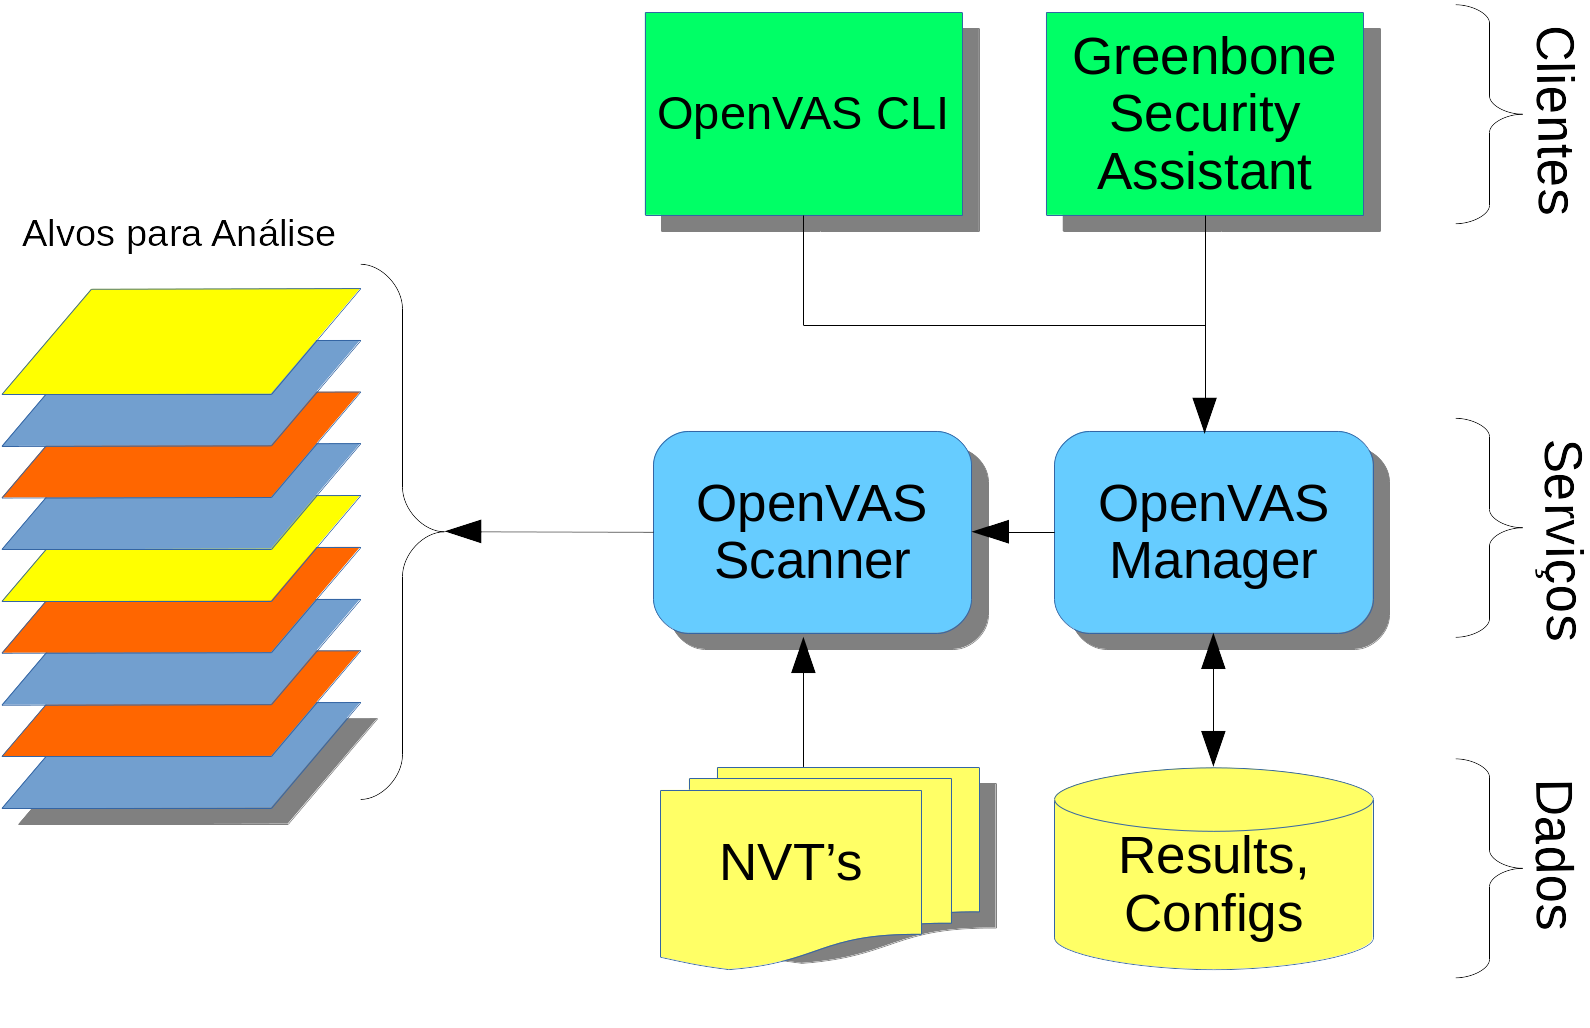
\includegraphics[width=0.90\textwidth]{figuras/Openvas Arquitetura.png}
    \caption{Arquitetura do \gls{OpenVAS} \cite{openvas}.}
    \label{fig:arquitetura:openvas}
\end{figure}

De acordo com \citeonline{vuldec}, a seguir serão descritos os componentes que formam a arquitetura do \gls{OpenVAS}:
\begin{itemize}
    \item \gls{GSA}: Fornece aos usuários uma interface web, na qual os mesmos podem gerenciar as configurações, criar varreduras e visualizar os relatórios de varreduras já executadas.
    \item \gls{OpenVAS} CLI: Cliente \gls{OpenVAS}, responsável por auxiliar o usuário através da interface de linha de comando, permitindo que usuários realizem as mesmas funções providas pelo \gls{GSA}, sem a necessidade de acessar uma interface gráfica.
    \item \gls{OpenVAS} \textit{Manager}: Serviço principal do \gls{OpenVAS}, controla o \textit{scanner} por um protocolo chamado de \gls{OTP}, além de ser responsável por armazenar a configuração e os resultados das varreduras. Também oferece funções adicionais, como por exemplo, agendamento de varreduras, geração de relatórios, entre outras, com uma ferramenta baseada em \gls{XML}, chamada de \gls{OMP}.
    \item \gls{OpenVAS} \textit{Scanner}: Núcleo da arquitetura do \gls{OpenVAS}, executa vários testes chamados de \gls{NVT}, estes testes verificam a presença de vulnerabilidades em sistemas. Os \gls{NVT}s são desenvolvidos utilizando \textit{scripts} da linguagem \gls{NASL}, e assim como o Nessus o \gls{OpenVAS} também possibilita a criação de seus próprios \textit{plugins} (\gls{NVT}) para a verificação de vulnerabilidades.
\end{itemize}

Como já citado anteriormente, o \gls{OpenVAS} é um \textit{framework} composto de vários serviços e ferramentas, segundo \citeonline{allen2014kali}, as ferramentas que compõem o \gls{OpenVAS} são mostradas na tebela~\ref{openvas-table}:
\begin{table}[H]
\centering
\caption{Ferramentas utilizadas pelo \gls{OpenVAS}}
\label{openvas-table}
\begin{tabular}{|l|l|}
\hline
\multicolumn{1}{|l|}{Ferramenta} & \multicolumn{1}{|l|}{Descrição}                                                                                                          \\ \hline
Amap                             & Ferramenta para detecção de protocolo de aplicações                                                                                     \\\hline
Ike-scan                         & \textit{Scanner} para detecção e testes de sistemas IPSec e VPN                                                                          \\\hline
Ldapsearch                       & Extrai informações dos dicionários LDAP                                                                                                 \\\hline
Nikto                            & Realiza análise de vulnerabilidades em servidores web                                                                                   \\\hline
Nmap                             & Realiza uma varredura das portas de um sistema                                                                                          \\\hline
Ovaldi                           & Realiza análise de vulnerabilidades em um sistema                                                                                       \\\hline
pnscan                           & Realiza uma varredura das portas de um sistema                                                                                          \\\hline
Portbunny                        & Realiza uma varredura das portas de um sistema                                                                                          \\\hline
Seccubus                         & Automatiza as varreduras realizadas pelo \gls{OpenVAS}                                                                                \\\hline
SLAD                             & Várias ferramentas de segurança (John-the-Ripper, Chkrootkit, ClamAV,  
\\&Snort,Logwatch, Tripwire, Lsof,Tiger, TrapWatch, e LM-sensors) \\\hline
                          
Snmpwalk                         & Extrai dados dos protocolos SNMP                                                                                                         \\\hline
Strobe                           & Realiza uma varredura das portas de um sistema                                                                                          \\\hline
w3af                             & Realiza ataques em aplicações web
\\ \hline
\end{tabular}
\end{table}

O \gls{OpenVAS} é uma ferramenta completa, podendo ser utilizada para analisar qualquer tipo de rede. Capaz de realizar desde simples varreduras de portas, utilizando ferramentas como Nmap, até quebras de senhas fracas, utilizando john-the-Ripper. Unindo tais características com o fato de ser uma ferramenta de código aberto e possuir uma comunidade forte e crescente, o \gls{OpenVAS} se destaca cada vez mais quando comparados com outros \textit{scanners} do gênero.


\subsection{Nmap}
Network mapper (Nmap), é uma ferramenta grátis e de código aberto, utilizada para monitorar e explorar redes de computadores. O \gls{Nmap} utiliza pacotes \gls{IP} para determinar quais dispositivos estão disponíveis na rede, quais serviços tais dispositivos oferecem, qual são os sistemas operacionais que os dispositivos estão executando, o \gls{MAC} dos dispositivos, entre outras características. O \gls{Nmap} é desenvolvido para monitorar redes com grandes quantidades de dispositivos, porém também funciona  em redes pequenas e/ou dispositivos únicos \cite{lyon2009nmap}.

O \gls{Nmap} também realiza  varreduras das portas de rede dos dispositivos alvos. A partir dessas varreduras são retornados os números das portas de rede, os protocolos de rede utilizados para as comunicações, as aplicações que estão executando e o estado das portas analisadas.

A saída dos dados do \citeonline{nmap} podem ser retornadas de cinco maneiras diferentes,  são elas:
\begin{itemize}
    \item Formato padrão: Todos os dados obtidos da varredura do \gls{Nmap} são mostrados no terminal de execução (\textit{stdout});
    \item Formato normal: Semelhante a saída padrão, porem com menos informações sobre as varreduras realizadas;
    \item Formato \gls{XML}: A varredura é convertida para um arquivo \gls{XML}, é uns dos formatos mais importantes de saída do \gls{Nmap}. O arquivo \gls{XML} pode ser facilmente analisado por programas para extrair informações, pode ser importado para bancos de dados, convertidos em arquivos \gls{HTML}, entres outras opções;
    \item Formato \textit{grep}: As informações sobre um determinado dispositivo são mostradas em apenas uma linha;
    \item Formato \textit{script kiddie}: Alguns caracteres são substituídos por números, não há nada especial neste formado de saída, apenas uma questão visual.
\end{itemize}

Deste modo, o \gls{Nmap} é uma das ferramentas mais poderosas para a análise de redes de computadores, com mais de 100 comandos que podem ser utilizados para realizar varreduras e obter diversas informações a respeito dos dispositivos analisados \cite{lyon2009nmap}.

Para a realização deste trabalho foram escolhida dois \textit{scanners} para serem utilizados, \gls{OpenVAS} e \gls{Nmap}, principalmente pelo fato de não possuírem custos para serem utilizados. Na próxima Seção será explicada a ferramenta de indexação e busca de texto Elasticsearch. 




%---------------------------------------------------%
\section{Elasticsearch}
ElasticSearch é uma ferramenta de busca  de texto de código aberto, desenvolvido na linguagem de programação Java\footnote{\url{https://www.java.com/pt_BR/}} e baseado em Apache Lucene\footnote{\url{https://lucene.apache.org/}}.  ElasticSearch foi desenvolvido com o objetivo de ser distribuído e escalável, tornando-se uma excelente ferramenta para trabalhar com \textit{big data}. É simples de instalar e a configuração padrão é suficiente para ser utilizada sem alterações \cite{Kononenko:2014:MMR:2597073.2597091}.

O Elasticsearch possui algumas características que o diferem do resto dos mecanismos de busca por texto \cite{elastic}, são elas:
\begin{itemize}
    \item Pesquisa e análise de dados em tempo real: Há apenas uma pequena latência do tempo em que um documento é indexado até o tempo em que ele pode ser pesquisado (normalmente um segundo);
    \item Distribuído e escalável: Um servidor Elasticsearch é chamado de nó, dois ou mais nós são chamados de \textit{cluster}. O Elasticsearch pode ser distribuído, analisando grandes quantidades de dados de maneira rápida e prática. A única mudança que precisa ser realizada nos arquivos de configurações é o nome do \textit{cluster}. O Elasticsearch se encarrega de encontrar os nós existentes e distribuir as informações entre os mesmos;
    \item Orientado a documentos: Os dados são armazenados em forma de documentos, um documento tem um tipo e os tipos estão dentro de um Índice. Os documentos são disponibilizados no formato \gls{JSON}, visando maior compatibilidade com várias linguagens de programação;
\end{itemize}


O Elasticsearch é capaz de realizar consultas com tempos muito inferiores quando comparado aos bancos de dados relacionais. Além disso,  possui um sistema de cacheamento, que possibilita que as consultas fiquem ainda mais rápidas a partir do segundo acesso.
O Elasticsearch possui \textit{plugins} que oferecem certas funcionalidades para a ferramenta de busca, visando melhorar a experiência dos usuários, como por exemplo o Kibana, que permite os usuários visualizarem as informações indexadas no motor de busca de forma gráfica e detalhada.
Tais características fazem do Elasticsearch uma poderosa ferramenta de busca, podendo ser utilizado em diversos conjuntos de dados diferentes.

 










%---------------------------------------------------% % Esse capítulo e nome é apenas uma sugestão.
% ATENÇÃO - veja com o seu orientador se você vai ter este capítulo e se este vai ter nome!
\chapter{Trabalhos Relacionados}
\label{cap:trabalhos:relacionados}

Neste capítulo serão apresentados os trabalhos relacionados com o presente trabalho, quais são suas similaridades, além de uma breve explicação de cada um.

\section{Vulnerability Assessment and Patching Management}

Em seu trabalho \citeonline{7489631} enfatiza a identificação e remoção de vulnerabilidades web, o artigo comenta principalmente de avaliação de vulnerabilidades (\textit{vulnerability assessment}), que é o processo de identificação, quantificação e classificação de vulnerabilidades. Primeiramente é explicado o processo de uma avaliação de vulnerabilidades, que é basicamente encontrar o sistema alvo e extrair informações. Nesse procedimento são realizados vários tipos de testes de penetração, como por exemplo, teste de caixa preta (\textit{black box testing}) e teste de caixa branca (\textit{white box testing}).

Durante esses testes, profissionais de segurança ou \textit{hackers}, tentam encontrar qualquer vulnerabilidade para depois explorá-la, e então ganhar acesso ao sistema. \citeonline{7489631} cita os principais motivos para a realização de um teste de penetração, são eles:
\begin{enumerate}
    \item Identificar os meios que um atacante pode obter acesso ao sistema;
    \item Saber qual é a maior ameaça do sistema, e corrigi-la assim que possível;
    \item Identificar as vulnerabilidades que sistemas automatizados não conseguem identificar;
    \item Identificar os riscos comerciais existentes. Uma empresa perderá a fé de seus clientes caso seus serviços fiquem indisponíveis.
    \item Verificar se o sistema responde bem aos ataques comuns.
    \item Mostrar que ataques podem ser realizados em sistemas vulneráveis, e assim convencer as organizações a investir mais em segurança.
\end{enumerate}

\citeonline{7489631} explica dois tipos de testes de penetração, os testes de penetração automáticos, no qual softwares procuram por vulnerabilidades em aplicações web, no final do teste é gerado um relatório contendo as vulnerabilidades e os métodos utilizados para resolver tais vulnerabilidades. E os testes de penetração manuais, no qual um profissional de segurança utiliza técnicas do mundo real, as mesmas utilizadas por \textit{hackers}, para explorar e ganhar acesso ao sistema, por exemplo, \textit{SQL Injection}, \gls{CSRF}, entre outras, o profissional em segurança utiliza seu conhecimento para encontrar, explorar e consertar as vulnerabilidades encontradas durante o processo de teste.

Também é discutido os principais tipos de vulnerabilidades baseadas em \gls{SQLI}, um tipo de vulnerabilidade na qual o atacante consegue ``injetar'' \gls{SQL}, em uma base de dados e conseguir informações restritas. Em seu trabalho \citeonline{7489631} introduz uma metodologia capaz de identificar declarações em aplicações \gls{PHP}, que podem estar vulneráveis para à \gls{SQLI}.

\citeonline{7489631} se relaciona com o presente trabalho quando utiliza teste de intrusão automático (automated pentesting) para encontrar vulnerabilidades. Testes de intrusão automáticos utilizam softwares para analisar dispositivos e identificar as vulnerabilidades existentes nos mesmos, por exemplo, \gls{OpenVAS} e Nessus.


\section{A Vulnerability Scanning Tool for Session Management Vulnerabilities}
\citeonline{vulnerabilityScanningTool} comenta a respeito das vulnerabilidades de gerenciamento de sessão (\textit{session management vulnerabilities} ) existentes em aplicações web. De modo resumido, vulnerabilidades de gerenciamento de sessão são muitas vezes vulnerabilidades que ainda estão sendo descobertas. O método de gerenciamento de sessão mais comum utiliza um identificador de sessão (\textit{session identifier}), esse \gls{SID} é um par ``nome=valor''. O valor é um número correspondente a uma sessão na web, o \gls{SID} deve ser enviado em cada requisição feita. Em aplicações web, o \gls{SID} geralmente é enviado em um campo oculto ou em um \textit{cookie} HTTP. Na maioria das vezes o gerenciamento de sessão é implementado incorretamente, o que acaba gerando as seguintes vulnerabilidades:
\begin{itemize}
    \item Correção de sessão (\textit{Session Fixation}): É uma vulnerabilidade que ocorre quando o atacante visita uma página web e recebe um \gls{SID}, após isso, o invasor manda uma \gls{URL} contendo o \gls{SID} para a vítima, quando a vítima visita a \gls{URL} e se autentica o \gls{SID} será o mesmo que o do atacante.
    \item \gls{CSRF}: Um invasor manda uma \gls{URL} manipulada para a vítima, quando visitado, a \gls{URL} faz uma requisição para o servidor web, sem nenhum reconhecimento da vítima.
    \item Insuficiente atributos \textit{Cookies}: O \textit{cookie}\footnote{cookies são pequenos arquivos de textos utilizados para que os sites recuperem informações sobre seus visitantes \cite{bishop2005introduction}.} geralmente serve como um contêiner para o \gls{SID}. Portanto o desenvolvedor deve tomar um cuidado especial quando estiver lidando com tais atributos, caso contrário, o atacante será capaz de roubar o \textit{cookie} contendo o \gls{SID}.
\end{itemize}

Para lidar para essas vulnerabilidades, \citeonline{vulnerabilityScanningTool} propõe uma solução de duas partes, a primeira é uma extensão para navegadores web, e a segunda parte é um \textit{plugin} desenvolvido para a ferramenta de análise de vulnerabilidades web Nikto. A primeira parte (extensão para navegadores web) serve como um identificador de vulnerabilidades único. E a segunda parte (Nikto) é usada para suportar o teste continuo, repetindo todo o processo feito na primeira parte automaticamente.

\citeonline{vulnerabilityScanningTool} acaba se assemelhando ao presente trabalho principalmente por dois motivos: A criação de uma ferramenta capaz de identificar vulnerabilidades utilizando um \textit{scanner},  e a automação da ferramenta.

\section{Penetration Testing in a Box}
\citeonline{Epling:2015:PTB:2885990.2885996} comenta sobre a importância dos testes de intrusão (\textit{pentest}) para qualquer empresa que dependa de uma infraestrutura de rede. Porém, esses testes possuem alguns empecilhos, por exemplo, o procedimento para executar um \textit{\gls{pentest}} pode demorar semanas ou até meses dependendo da infraestrutura da rede a ser analisada e da quantidade de informações que os clientes desejam, aumentando de maneira significativa o seu custo. Tal custo pode ser um problema para as pequenas empresas, que muitas vezes não possuem verbas necessárias para realizar um teste completo. Portanto, \citeonline{Epling:2015:PTB:2885990.2885996} menciona a existência de dispositivos, disponíveis comercialmente, que possuem todas as ferramentas necessárias para realizar um teste de intrusão de maneira confiável.


Deste modo, \citeonline{Epling:2015:PTB:2885990.2885996} propõe a criação de um dispositivo barato, capaz de realizar \textit{\gls{pentest}} utilizando microcomputadores Raspberry Pi\cite{raspberry}. Permitindo que empresas que não possuem orçamentos necessário para contratar firmas de segurança consigam realizar avaliações completas de suas infraestruturas. \citeonline{Epling:2015:PTB:2885990.2885996} chama deu dispositivo de \textit{Pentest Box}. Quando conectado às redes internas, o \textit{Pentest Box} possibilita que administradores acessem sua interface web remotamente, podendo realizar varreduras, e avaliação de toda rede.

\citeonline{Epling:2015:PTB:2885990.2885996} se assemelha com o presente trabalho quando utiliza \textit{scanners} de vulnerabilidades para realizar a varredura das redes monitoradas. Além disso, o \textit{Pentest Box} automatiza o processo reconhecimento da rede local, tal automatização é um dos objetivos do trabalho futuro da ferramenta proposta.
 
 % Esse capítulo e nome é apenas uma sugestão.
% ATENÇÃO - veja com o seu orientador se você vai ter este capítulo e se este vai ter nome!
\chapter{Proposta e metodologia}
\label{cap:proposta}
Neste trabalho é proposto a criação de uma arquitetura que seja capaz de auxiliar na detecção e visualização de vulnerabilidades em redes de computadores. A ideia fundamental é utilizar sensores, com o objetivo de obter a maior quantidade de informações disponíveis a respeito dos dispositivos que serão analisados, criando perfis e utilizando esses perfis para facilitar a administração da rede. Além disso, todas essas informações serão mostradas de maneira gráfica, facilitando para o usuário o entendimento dos resultados obtidos. Para validar a arquitetura proposta será implementada uma ferramenta, na qual será utilizada dois \textit{scanners} para obter informações a respeito da rede analisada, são eles: \gls{OpenVAS} e \gls{Nmap}. As informações obtidas serão utilizadas para auxiliar no gerenciamento e manutenção da rede monitorada. 

A sequência deste capítulo detalha a metodologia utilizada para cumprir o objetivo proposto neste trabalho. Além de explicar detalhadamente a implementação da ferramenta comentada anteriormente.
%---------------------------------------------------%
\section{Metodologia}
A complexidade das redes de computadores aumentou consideravelmente nos últimos anos. De acordo com \citeonline{Gawron:2015:AVD:2799979.2799986} tal complexidade é tão grande que se tornou praticamente impossível gerenciar os riscos de segurança manualmente. Deste modo, ferramentas que auxiliam os administradores de redes na realização de tal gerenciamento tornaram-se necessárias, como por exemplo os \textit{scanners} de vulnerabilidade, \textit{scanners} de rede, entre outras. Porém, os \textit{scanners} tendem a gerar quantidades significativas  de informações, demandando grande tempo dos administradores de redes para analisar e entender tais informações.

Deste modo, a arquitetura proposta deve auxiliar tanto na detecção das vulnerabilidades quanto na visualização dos dados retornados. Tal arquitetura é ilustrada na Figura~\ref{fig:projeto:etapas}.
\begin{figure}[H]
    \centering
    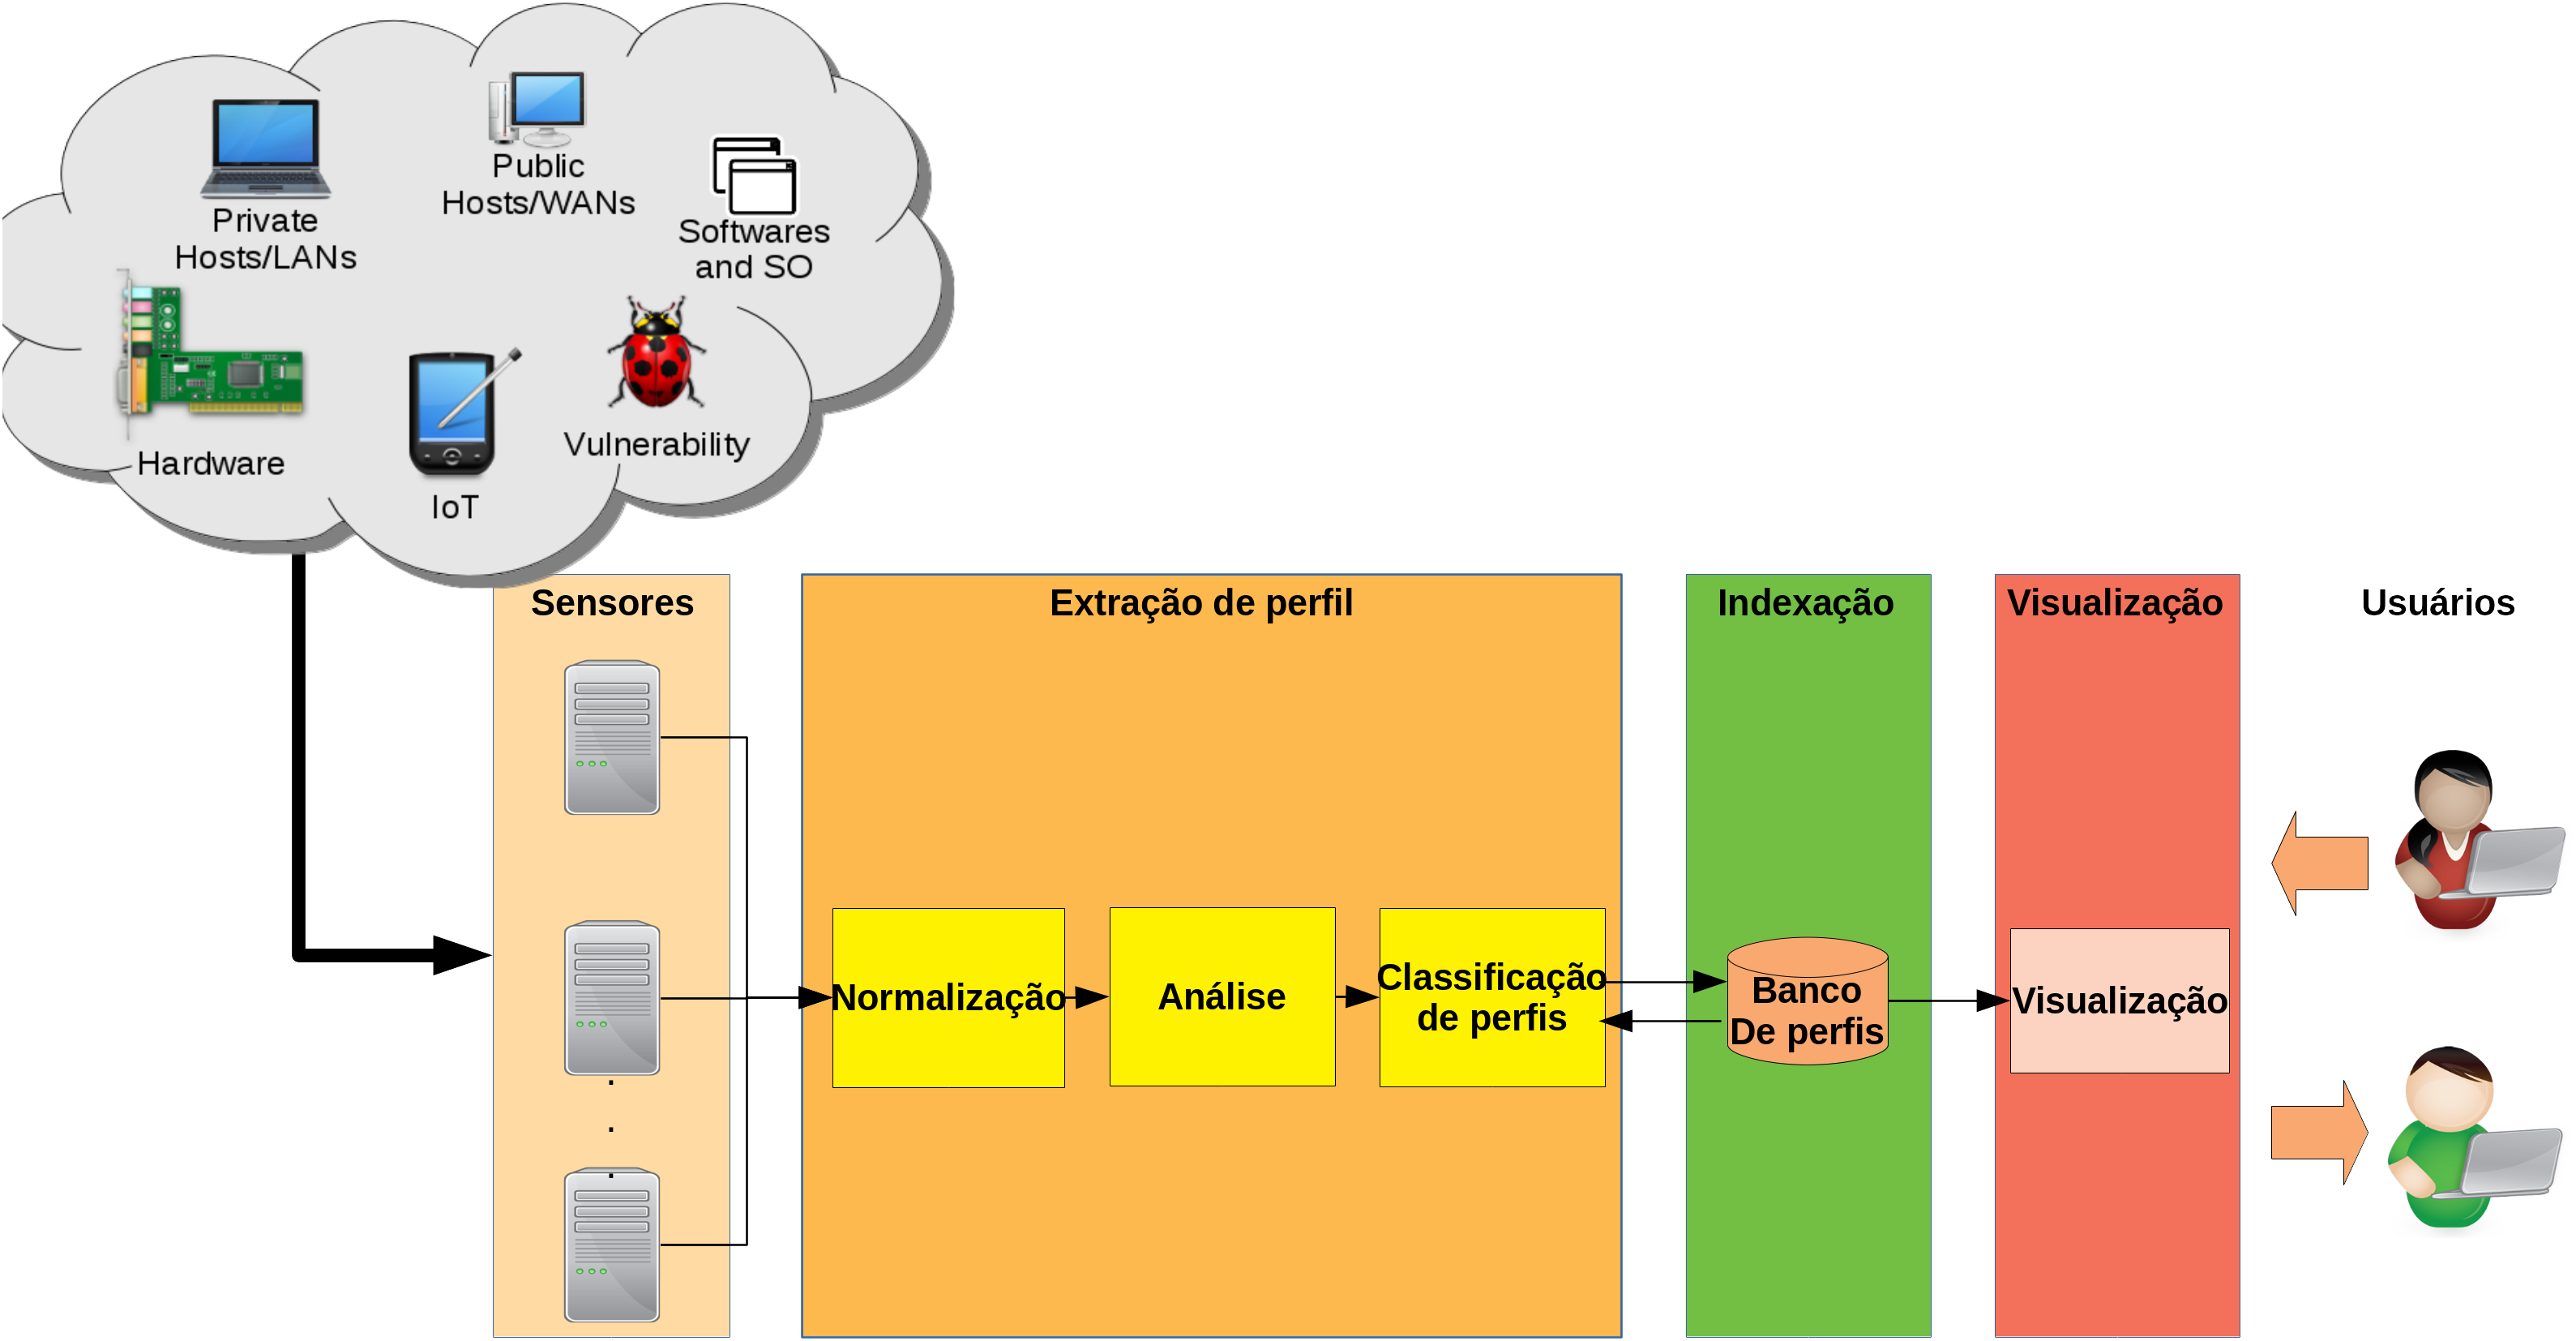
\includegraphics[width=0.90\textwidth]{figuras/tcc.png}
    \caption{Arquitetura proposta.}
    \label{fig:projeto:etapas}
\end{figure}
Conforme a Figura~\ref{fig:projeto:etapas} a arquitetura é composta dos seguintes elementos:
\begin{enumerate}
\item Sensores: Devem coletar o máximo de informações possíveis a respeito dos dispositivos analisados. Vários sensores podem ser utilizados, aumentando a diversidade dos dados coletados.
\item Extração de perfil: Como vários sensores podem ser utilizados na análise dos dispositivos, as informações retornadas devem ser normalizadas, assim, é possível analisar essas informações e extrair características a respeito dos dispositivos analisados, como por exemplo, softwares que estão executando nos dispositivos, sistemas operacionais utilizados, \gls{IP}, entre outras. Essas características serão utilizadas para criação/atualização de perfis, que serão divididos em três grupos, de acordo com a severidade das  vulnerabilidades encontradas nos mesmos, são eles: ``Perfis de alto risco'', ``Perfis de médio risco'', ``Perfis de baixo risco''. Os perfis de alto risco possuem severidades mais graves, portanto possuem uma chance maior de serem invadidos. Os perfis de médio risco, possuem vulnerabilidades de níveis médios, desse modo possuem menos chances de serem invadidos. E os perfis de baixo risco praticamente não possuem vulnerabilidades potenciais para uma invasão. A classificação dos perfis em seus devidos grupos é feita utilizando o valor do \gls{CVSS} de cada vulnerabilidade encontrada no perfil analisado. O \gls{CVSS} é uma métrica utilizada para calcular a severidade de vulnerabilidades. Após a classificação dos perfis os mesmos serão indexados em uma base de dados.
\item Indexação: Os perfis obtidos na extração de perfis serão indexados em um banco de dados, quando uma nova análise da rede é feita as informações nos perfis serão atualizadas e os novos dados serão indexados ao banco juntamente com a sua data. Deste modo será possível manter um histórico dos perfis, tal histórico poderá ser visualizado pelos usuários, para verificar se novas vulnerabilidades foram encontradas desde a última varredura realizada. Essas informações serão utilizadas para gerar visualizações a respeito dos ambientes analisados, auxiliando os usuários da ferramenta na administração da rede monitorada.
\item Visualização: Os usuários do sistemas poderão observar os dados obtidos através de uma interface, visando melhor entendimento das informações coletadas, como por exemplo, obter uma visão geral da topologia da rede analisada, visualizar as informações sobre os dispositivos, entre outras.
\end{enumerate}


Para validar a arquitetura proposta uma ferramenta será implementada. A ferramenta utilizará dois sensores, um para obter informações vindas do \textit{scanner} de rede \gls{Nmap} e outro para capturar as informações do \textit{scanner} de vulnerabilidade \gls{OpenVAS}. O \gls{Nmap} será utilizado para obter as portas de redes abertas, as aplicações que estão executando nessas portas, os sistemas operacionais e o \gls{MAC} dos dispositivos. O \gls{MAC} é um valor único, associado à interface de comunicação utilizada pelo dispositivo para se conectar a rede. Tal valor será utilizado como uma identificação única dos dispositivos analisados. O outro sensor será o \gls{OpenVAS} no qual será utilizado para obter as vulnerabilidades existentes nos dispositivos. Essas informações serão retornadas em um arquivo \gls{XML}.

O arquivo \gls{XML} gerado anteriormente será analisado, e a partir das informações encontradas neste arquivo serão gerados os perfis dos dispositivos. Um \textit{script} implementado na linguagem de programação Python\footnote{\url{https://www.python.org/}} será utilizado para analisar o arquivo \gls{XML} e criar os perfis dos dispositivos. O \textit{script} percorre as \textit{tags} \gls{XML} e coleta as informações contidas nas mesmas. As vulnerabilidades retornadas pelo \gls{OpenVAS} marcadas como ``\textit{log}'' não serão utilizadas, pois são informações semelhantes às retornadas pelo \gls{Nmap}.  O \textit{script} retorna as informações filtradas no formato \gls{JSON}. Tal formato foi escolhido devido a sua simplicidade e a facilidade de integração com o motor e busca Elasticsearch, que será utilizado neste trabalho. O código a seguir apresenta um exemplo de arquivo obtido no término da execução do \textit{script}.


%\item Obter informações dos sistemas: Sensores devem obter o máximo de informações possíveis a respeito os sistemas analisados, vários sensores podem ser utilizados nesta etapa da arquitetura, como por exemplo, \textit{scanners} de rede, \textit{scanners} de vulnerabilidades, ferramentas para análise do fluxo de dados na rede, entre outras, depois de obter as informações, as mesmas devem ser normalizadas, para que se possa extrair características que serão utilizadas para ; 
%\item Extração de perfis: Toda informação obtida na etapa anterior será normalizada, para que se consiga analisar essas informações e extrair características, que serão usadas para montar um perfil para cada sistema analisado. Os perfis podem ser divididos em dois grupos, são eles: ``Perfis vulneraveis'' e ``Perfis normais''. Os ``Perfis vulneraveis'' são informações sobre sistemas que de algum modo já sofreram intrusão ou outro tipo de ataque bem sucedido. O sistema Horus será responsável por ceder os sistemas que já sofreram ataques(>>melhorar). Os ``Perfis normais'' possuem informações dos sistemas analisados pelo sensores que não tenham sidos explorados. Estes perfis serão utilizados para gerar visualizações sobre o ambiente analisado, realizar comparações de similaridade de perfis, entre outras funções;
%\item Indexação: Os perfis obtidos na etapa anterior serão indexados em um motor de busca, onde serão feitas as comparações de similaridade entre perfis do grupo ``Perfis vulneraveis'' com perfis do grupo ``Perfis normais'', além disso, as informações indexadas serão utilizadas para gerarem uma visualização mais detalhada do ambiente analisado; 
%\item Comparação de perfis: Comparar perfis de dispositivos analisados com os perfis vulneráveis;
%\item Visualização de dados: Mostrar os dados obtidos para o usuário.
%As etapas da arquitetura serão explicadas detalhadamente a seguir.


%O arquivo \gls{XML} gerado na etapa 1 precisa ser filtrado e organizado de maneira que seja montado um perfil para cada dispositivo analisado. Portanto, na etapa 2, o \gls{XML} é filtrado visando diminuir a quantidade dos dados retornados pelos \textit{scanners}, tal filtragem é realizada utilizando um \textit{script}, implementado na linguagem de programação python\footnote{\url{https://www.python.org/}}. O \textit{script} percorre as \textit{tags} \gls{XML} e coleta as informações contidas nas mesmas. As vulnerabilidades retornadas do \gls{OpenVAS} marcadas como ``\textit{log}'' serão desconsideradas pois são informações semelhantes as retornadas pelo \gls{Nmap}.  O \textit{script} retorna as informações filtradas no formato \gls{JSON}, tal formato foi escolhido devido a sua simplicidade e a facilidade de integração com o banco de dados não-relacional ElasticSearch, que armazena os dados no formato  \gls{JSON}. A Figura~\ref{fig:formato:json} apresenta o arquivo obtido após a filtragem das informações.
\begin{lstlisting}[style=json, label=arquivo:json:output, caption={Exemplo de arquivo \gls{JSON} gerado a partir das informações.}, basicstyle=\scalefont{0.6}]
{
      "MAC":"90:2B:34:3C:7C:97",
      "OS":"Linux 3.2 - 4.6",
      "Ports":{
         "22":"OpenSSH 7.2p2 Ubuntu 4ubuntu2.1 (Ubuntu Linux; protocol 2.0)",
         "80":"Apache httpd 2.2.22 ((Ubuntu))",
         "443":"lighttpd 1.4.13"
      },
      "Hardware":"Giga-byte Technology",
      "vuls":[
         {
            "Threat":"High",
            "IP":"172.16.2.136",
            "CVSS":"7.1",
            "Protocol":"tcp",
            "Port":"80",
            "OID":"1.3.6.1.4.1.25623.1.0.800827",
            "Name":"Apache 'mod_proxy_http.c' Denial Of Service Vulnerability",
            "Impact":"Successful exploitation will allow remote attackers to cause Denial of Service to the legitimate user by CPU consumption. Impact Level: Application",
            "CVE":"CVE-2009-1890",
            "References":"http://secunia.com/advisories/35691 http://www.vupen.com/english/advisories/2009/1773",
            "Date":"2017-09-19T01:17:47Z"
         }]
}
\end{lstlisting}

O \gls{JSON} obtido para a criação dos perfis no banco contém os seguintes campos:
\begin{itemize}
    \item \gls{MAC}: Valor único, utilizado para identificar um dispositivo de rede perante aos outros;
    \item \gls{OS}: Sistema operacional executando no dispositivo;
    \item \textit{Ports} (Portas): Portas de rede encontradas abertas;
    \item Hardware: Hardware do dispositivo;
\end{itemize}
Além dessas informações, também existe um vetor de vulnerabilidades, com os seguintes campos:
\begin{itemize}
    \item \textit{Threat} (ameaça): O nível de ameaça que tal vulnerabilidade representa para o sistema em qual foi detectada, os \textit{scanners} testados no presente trabalho possuem 4 níveis de ameaças,  alto(\textit{high}) , médio (\textit{medium}),  baixo (\textit{low}) e informações  (\textit{logs}), esses níveis são determinados utilizando a pontuação obtida durante o cálculo do \gls{CVSS}.  Os \textit{logs} não são considerados ameaças, são informações que o \textit{scanner} conseguiu adquirir do sistema alvo (sistema operacional, versões de aplicativos instalados, entre outras);
    \item \gls{CVSS}: Uma métrica padrão para calcular o nível de severidade das vulnerabilidades. O cálculo é feito levando em consideração a facilidade para explorar a vulnerabilidade e o impacto da exploração. Após o cálculo, uma pontuação é atribuída a tal vulnerabilidade, podendo ir de 0 até 10, onde 10 é considerado severidade máxima \cite{cvss};
    \item \textit{Protocol} (protocolo): Protocolo de comunicação de rede utilizado quando a vulnerabilidade foi detectada;
    \item \textit{Port} (porta): Porta de rede em qual a vulnerabilidade foi detectada;
    \item OID: Identificador único de vulnerabilidades dentro da base de dados do \gls{OpenVAS};
    \item \textit{Name} (nome): Nome da vulnerabilidade;
    \item \textit{Impact} (impacto): Impacto para o sistema caso ocorra a exploração da vulnerabilidade;
    \item \gls{CVE}: Uma base de dados internacional contendo características de vulnerabilidades descobertas\footnote{\url{https://cve.mitre.org/}};
    \item \textit{References} (referências): Informações a respeito das vulnerabilidades;
    \item \textit{Date} (data): A data exata contendo dia, mês, ano, horas, minutos e segundos na qual a vulnerabilidade foi detectada.
\end{itemize}

O \gls{JSON} será persistido em um banco de dados. Para implementar este trabalho foi escolhido o motor de busca Elasticsearch. Para a visualização dos dados será utilizado o \textit{plugin} Kibana. A partir dos dados contidos no Elasticsearch, através de uma interface web, o usuário é capaz de analisar todas as informações a partir de gráficos dos mais variados estilos, como por exemplo, gráfico de barras, gráficos de linhas, entre outros.


Deste modo, a ferramenta é capaz de simplificar a análise de dos dados obtidos através dos \textit{scanners} utilizados, auxiliando os usuários na detecção e visualização de vulnerabilidades, facilitando também no gerenciamento de redes de computadores.


%--------------------------------------------------%
\section{Cronograma de Atividades}

Nesta seção são apresentadas as atividades a serem desenvolvidas para a execução da proposta. O cronograma de realização das tarefas é apresentado na Tabela~\ref{tab:cronograma}.


Os seguintes itens fazem parte do cronograma:

\begin{enumerate}
\item \textbf{Estudo da ferramenta ElasticSearch.}
\item \textbf{Persistência dos dados no banco.}
\item \textbf{Implementação da Ferramenta proposta.}
\item \textbf{Estudo da ferramenta Kibana.}
\item \textbf{Realização dos experimentos utilizando a ferramenta proposta.}
\item \textbf{Teste e análise dos resultados obtidos.}
\item \textbf{Escrita do TCC2}
\item \textbf{Entrega do TCC 2.}
\item \textbf{Apresentação do TCC 2.}
\end{enumerate}




% Please add the following required packages to your document preamble:
% \usepackage{multirow}
% Please add the following required packages to your document preamble:
% \usepackage{multirow}
\begin{table}[H]
\renewcommand{\arraystretch}{1.3}
\centering
\caption{Cronograma das Atividades}
\label{tab:cronograma}
\scalefont{0.9}
\begin{tabular}{|l|l|l|l|l|l|l|l|l|}
\hline
\multicolumn{1}{|c|}{\multirow{2}{*}{\textbf{Atividade}}} & \multicolumn{6}{c|}{\textbf{2018}}         \\ \cline{2-7} 
\multicolumn{1}{|c|}{}                           & \textbf{Jan} & \textbf{Fev} & \textbf{Mar} & \textbf{Abr} & \textbf{Mai} & \textbf{Jun} \\ \hline
\textbf{1}                                                & X   &     &     &     &     &     \\ \hline
\textbf{2}                                                &  X   &    &     &     &     &     \\ \hline
\textbf{3}                                                &  X   &  X   & X    &    X& X    &     \\ \hline
\textbf{4}                                                &     &    X &     &     &     &     \\ \hline
\textbf{5}                                                &     &     &     X&  X   &     &     \\ \hline
\textbf{6}                                                &     &     &     &    X &    X &     \\ \hline
\textbf{7}                                                &   X  &   X  &X     &   X  & X    & X    \\ \hline
\textbf{8}                                                &     &     &     &     &     &     X\\ \hline
\textbf{9}                                                &     &     &     &     &     &     X\\ \hline
\end{tabular}
\end{table}
 % Esse capítulo e nome é apenas uma sugestão (bom para TCC 1).
\include{capitulos/cap-metodologia} % Esse capítulo e nome é apenas uma sugestão.
\include{capitulos/cap-experimentos-resultados} % Esse capítulo e nome é apenas uma sugestão.
\chapter{Conclusões parciais}
Como visto, a detecção e visualização de vulnerabilidades são processos trabalhosos no gerenciamento de redes de computadores. Tais processos podem gerar grandes quantidades de informações e acabar demandando um grande tempo de análise dos administradores de redes. A arquitetura proposta mostra potencial para auxiliar tanto  na detecção quanto na  visualização de vulnerabilidades. Além disso, a arquitetura também pode facilitar o gerenciamento da rede em geral, a criação dos perfis, juntamente com uma interface de visualização pode fornecer para o usuário uma grande quantidade de informações a respeito do ambiente analisado.

O próximo passo deste trabalho será a implementação de uma ferramenta seguindo a arquitetura proposta. Os \textit{scanners} \gls{OpenVAS} e \gls{Nmap} serão utilizados para obter as informações da rede monitorada. As informações serão normalizadas e analisadas por um \textit{script} implementado na linguagem de programação Python. Os perfis criados serão indexados no motor de busca Elasticsearch e a visualização dos dados serás realizada com o \textit{plugin} Kibana. A ferramenta será testada em um período de dois meses, será analisado o tempo que a ferramenta leva para realizar uma varredura completa na rede, as informações capturadas pelas varreduras realizadas e a visualização gráfica das informações obtidas.
 % Esse capítulo e nome é apenas uma sugestão.

% Apendices.
%\appendix
%\include{postextual/ape-instalacao-ferramentas}

%bibliografia
\bibliographystyle{abntex2-alf}
\bibliography{main} % geração automática das referências a partir do arquivo main.bib

\backmatter
\end{document}
